%! Author = Сергей
%! Date = 27.02.2023

% Preamble
\documentclass[11pt]{article}

% Packages
\usepackage[utf8]{inputenc}
\usepackage{tikz}
\usetikzlibrary{shapes.geometric, arrows}

% Tikz styles
\tikzstyle{startstop} = [
    rectangle, rounded corners,
    minimum width=3cm, minimum height = 1cm,
    text centered,
    draw=black, fill=red!30
]
\tikzstyle{io} = [
    trapezium, trapezium left angle=70, trapezium right angle=110,
    minimum width=3cm, minimum height = 1cm,
    text centered,
    draw=black, fill=blue!30
]
\tikzstyle{process} = [
    rectangle,
    minimum width=3cm, minimum height = 1cm,
    text centered, text width=3cm,
    draw=black, fill=orange!30
]
\tikzstyle{decision} = [
    diamond,
    minimum width=3cm, minimum height = 1cm,
    text centered,
    draw=black, fill=green!30]
\tikzstyle{arrow} = [thick,->,>=stealth]

% Document
\begin{document}
    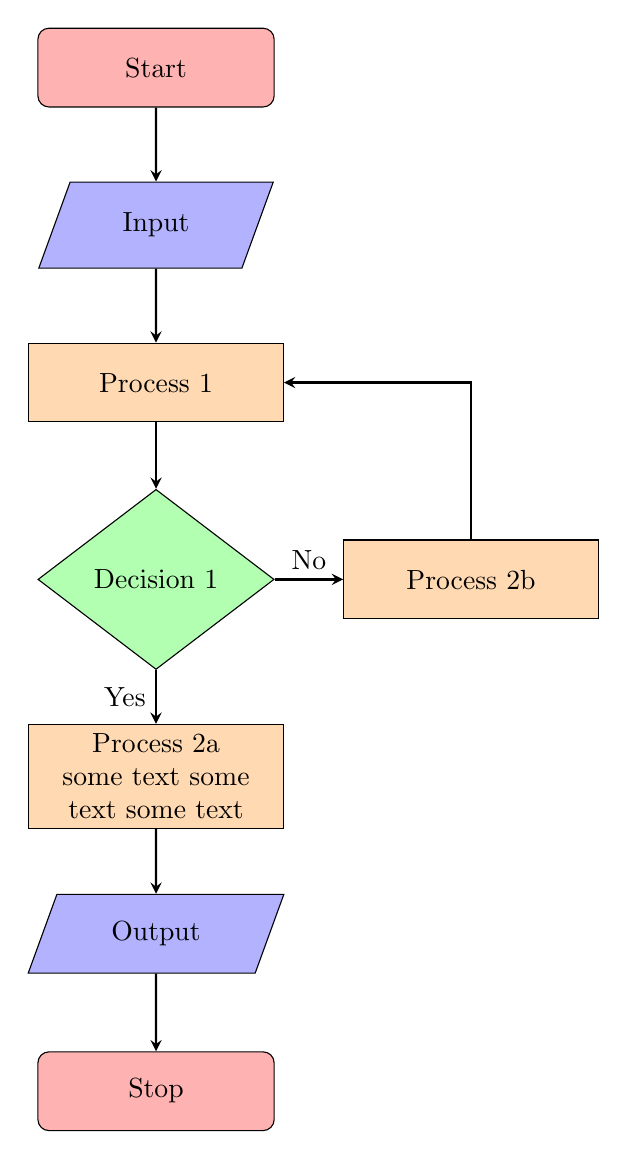
\begin{tikzpicture}[node distance=2cm]
        % Draw blocks
        \node (start) [startstop] {Start};
        \node (i1) [io, below of=start] {Input};
        \node (p1) [process, below of=i1] {Process 1};
        \node (d1) [decision, below of=p1, yshift=-0.5cm] {Decision 1};
        \node (p2a) [process, below of=d1, yshift=-0.5cm] {Process 2a some text some text some text};
        \node (p2b) [process, right of=d1, xshift=2cm] {Process 2b};
        \node (o1) [io, below of=p2a] {Output};
        \node (stop) [startstop, below of=o1] {Stop};

        % Draw arrows
        \draw [arrow] (start) -- (i1);
        \draw [arrow] (i1) -- (p1);
        \draw [arrow] (p1) -- (d1);
        \draw [arrow] (d1) -- node[anchor=east] {Yes} (p2a);
        \draw [arrow] (d1) -- node[anchor=south] {No} (p2b);
        \draw [arrow] (p2b) |- (p1);
        \draw [arrow] (p2a) -- (o1);
        \draw [arrow] (o1) -- (stop);
    \end{tikzpicture}
\end{document}